\section{Numerical Tests}
\label{sec:numerical}

\subsection{Problems with Known Smooth Solutions}
\label{sec:smoothProblems}

To compare the accuracy of the IMEX schemes, we present results from smooth problems in streaming, absorption, and scattering dominated regimes in one spatial dimension.  
In all tests, we employ the maximum entropy closure in the low occupancy limit (i.e., the Minerbo closure).  

\subsubsection{Sine Wave: Streaming}

The first test involves the streaming part only, and does not include any collisions ($\sigma_{\Ab}=\sigma_{\Scatt}=0$).  
We consider a periodic domain $D=\{x:x\in[0,1]\}$, and let the initial condition be given by
\begin{equation}
  \cJ(x,t=0)=\cH_{x}(x,t=0)=0.5+0.49\times\sin\big(2\pi\,x\big).  
  \label{eq:initialConditionStreaming}
\end{equation}
We evolve until $t=10$, when the sine wave has completed 10 crossings of the computational domain.  
We use polynomials of degree $k=2$ for the spatial discretization (third-order spatial accuracy), and set the time step as $\Delta t = $.  
We vary the number of elements from $??$ to $??$ and compute errors for various time stepping schemes.  

\ee{Include figure of error versus number of elements for various schemes.}

\begin{figure}[h]
  \centering
    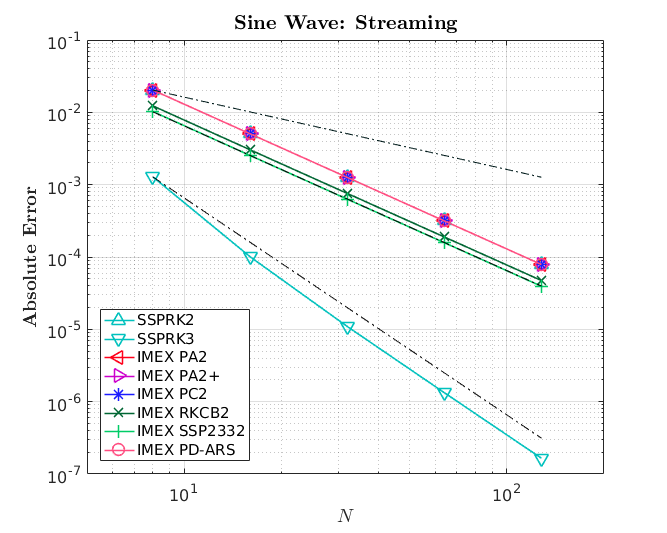
\includegraphics[width=\textwidth]{figures/SineWaveStreaming}
   \caption{Sine Wave Streaming}
  \label{fig:SineWaveStreaming}
\end{figure}

\subsubsection{Sine Wave: Damping}

The next test we consider, adapted from \cite{skinnerOstriker_2013}, consists of a sine wave propagating with unit speed in a purely absorbing medium ($f_{0}=0$, $\sigma_{\Scatt}=0$), which results in exponential damping of the wave amplitude.  
We consider a periodic domain $D=\{x:x\in[0,1]\}$, and let the initial condition ($t=0$) be given as in Eq.~\eqref{eq:initialConditionStreaming}.  
For a constant absorption opacity $\sigma_{\Ab}$, the analytical solution at $t>0$ is given by
\begin{equation}
  \cJ(x,t)=\cJ_{0}(x-t)\times\exp(-\sigma_{\Ab} t)
  \quad\text{and}\quad
  \cH_{x}(x,t)=\cJ(x,t),
\end{equation}
where $\cJ_{0}(x)=\cJ(x,0)$.  

We compute numerical solutions for three values of the absorption opacity ($\sigma_{\Ab}=0.1$, $1$, and $10$), and adjust the end time $t_{\mbox{\tiny end}}$ so that $\sigma_{\Ab}t_{\mbox{\tiny end}}=10$, and the initial condition has been damped by factor $e^{-10}$.  
Thus, for $\sigma_{\Ab}=0.1$ the sine wave crosses the domain 100 times, while for $\sigma_{\Ab}=10$, it crosses the grid once.  

Figure~\ref{fig:SineWaveDamping} shows convergence results obtained for the various values of $\sigma_{\Ab}$, using various IMEX schemes.  
Results for $\sigma_{\Ab}=0.1$, $1$, and $10$ are plotted with red, green, and blue lines, respectively.  

\begin{figure}[h]
  \centering
    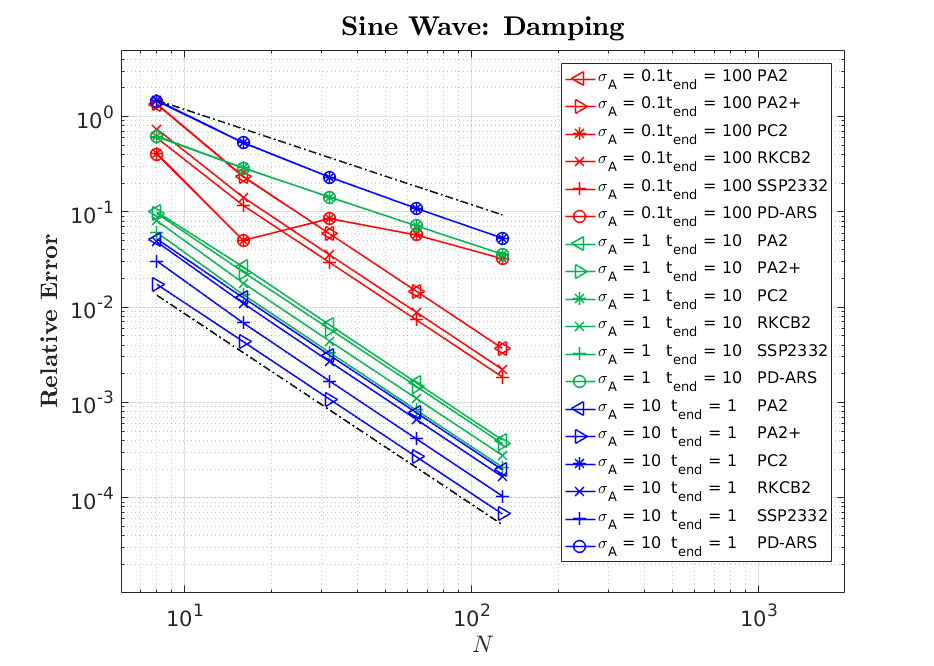
\includegraphics[width=\textwidth]{figures/SineWaveDamping}
   \caption{Sine Wave Damping}
  \label{fig:SineWaveDamping}
\end{figure}

\subsubsection{Sine Wave: Diffusion}

The final test with known smooth solutions, adopted from \cite{radice_etal_2013}, is diffusion of a sine wave in a purely scattering medium ($f_{0}=0$, $\sigma_{\Ab}=0$).  
The computational domain $D=\{x:x\in[-3,3]\}$ is periodic, and the initial condition is given by
\begin{equation}
  \cJ_{0}(x)=0.5+0.49\times\sin\big(\pi\,x/3\big)
  \quad\text{and}\quad
  \cH_{x,0}
  =-\f{1}{3\sigma_{\Scatt}}\pderiv{\cJ_{0}}{x}.  
\end{equation}

\begin{figure}[h]
  \centering
  \begin{tabular}{cc}
    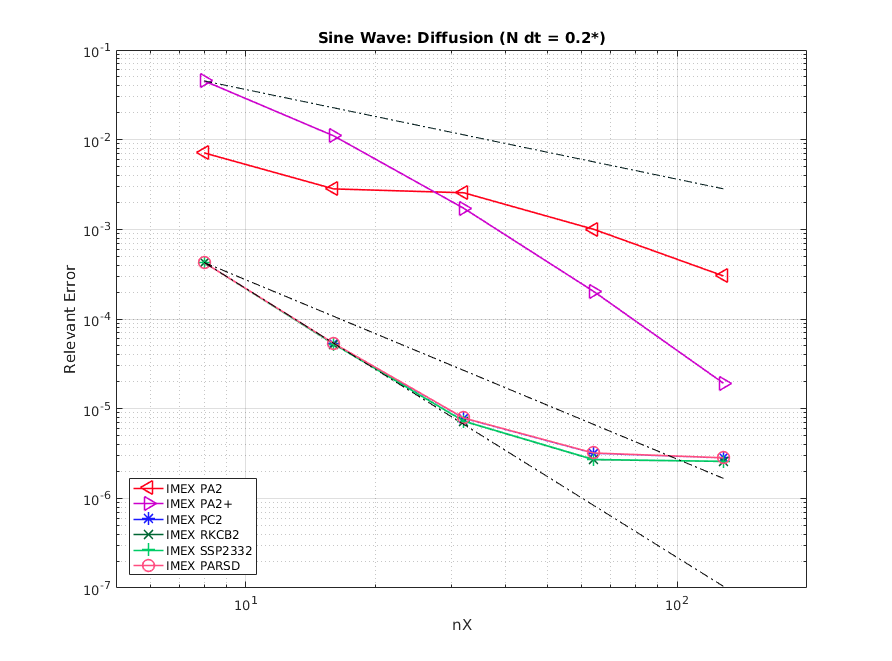
\includegraphics[width=0.5\textwidth]{figures/SineWaveDiffusionN} &
    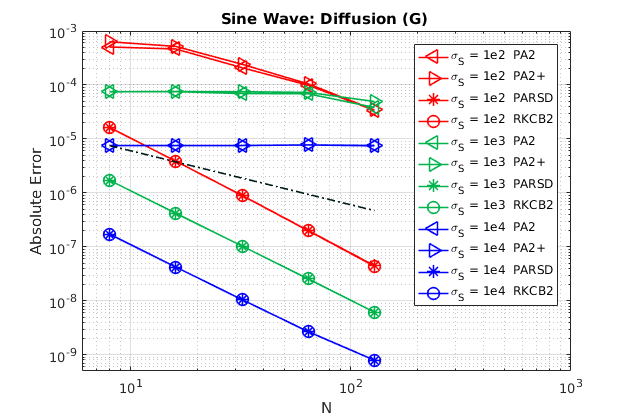
\includegraphics[width=0.5\textwidth]{figures/SineWaveDiffusionG}
    \end{tabular}
   \caption{Sine Wave Diffusion}
  \label{fig:SineWaveDiffusion}
\end{figure}

\subsection{Packed Beam}

Next we consider a one-dimensional test with discontinuous initial conditions.  
The computational domain is $D=\{x:x\in[-1,1]\}$, and the initial condition is obtained from a distribution function given by
\begin{equation}
  f(x,\mu)
  =\left\{
  \begin{array}{cl}
    1        & \text{if} ~ x\le x_{\mbox{\tiny D}}, ~ \mu\ge\mu_{\mbox{\tiny D}} \\
    \delta & \text{if} ~ x\le x_{\mbox{\tiny D}}, ~ \mu<   \mu_{\mbox{\tiny D}} \\
    \delta & \text{otherwise},
  \end{array}
  \right.
\end{equation}
so that $\vect{\cM}=\big(0.5\,(1+\delta),0.25\,(1-\delta)\big)^{T}$ for $x\le x_{\mbox{\tiny D}}$, and $\vect{\cM}=\big(\delta,0\big)^{T}$ for $x> x_{\mbox{\tiny D}}$, where $\delta>0$ is a small parameter ($\delta\ll1$).  
We let $\delta=10^{-8}$.  
\begin{figure}[h]
  \centering
  \begin{tabular}{cc}
    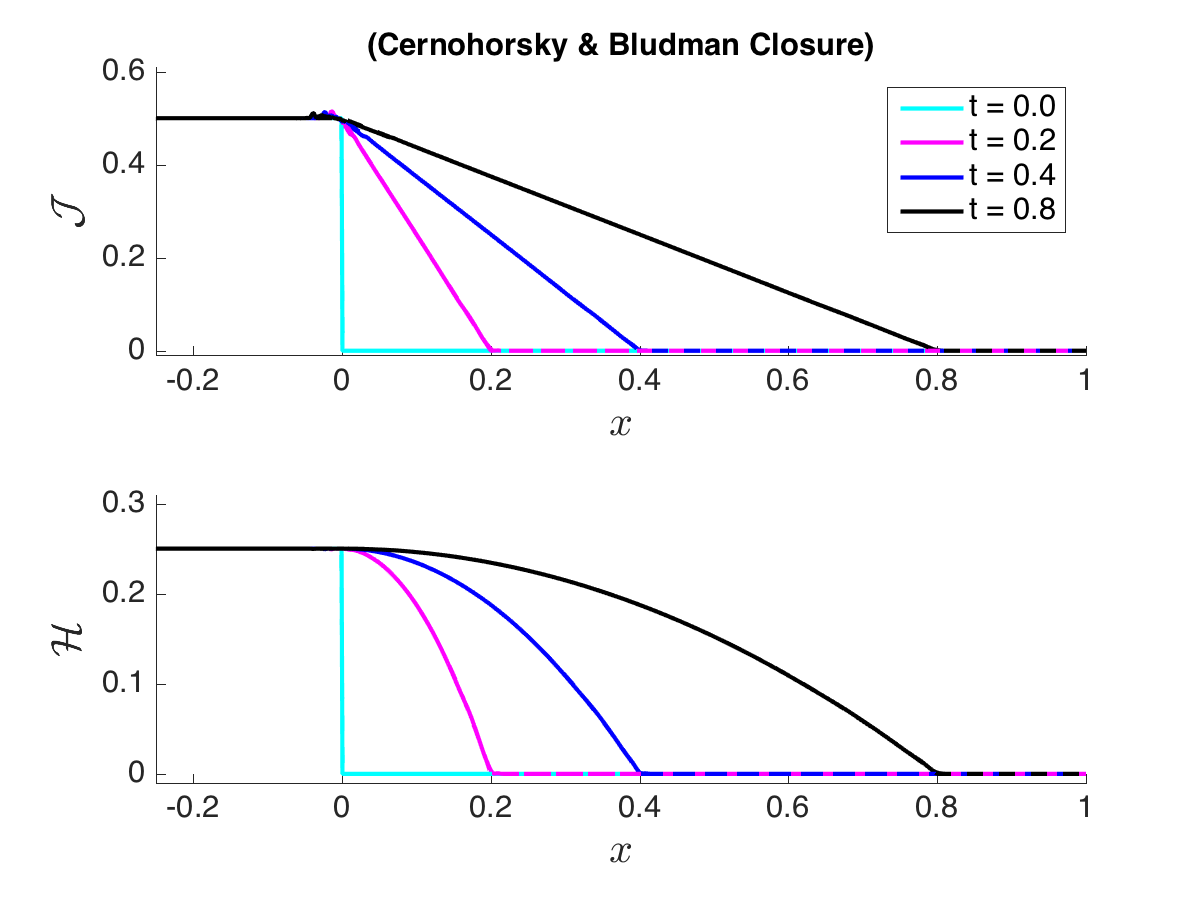
\includegraphics[width=0.5\textwidth]{figures/PackedBeam_ME_CB}
    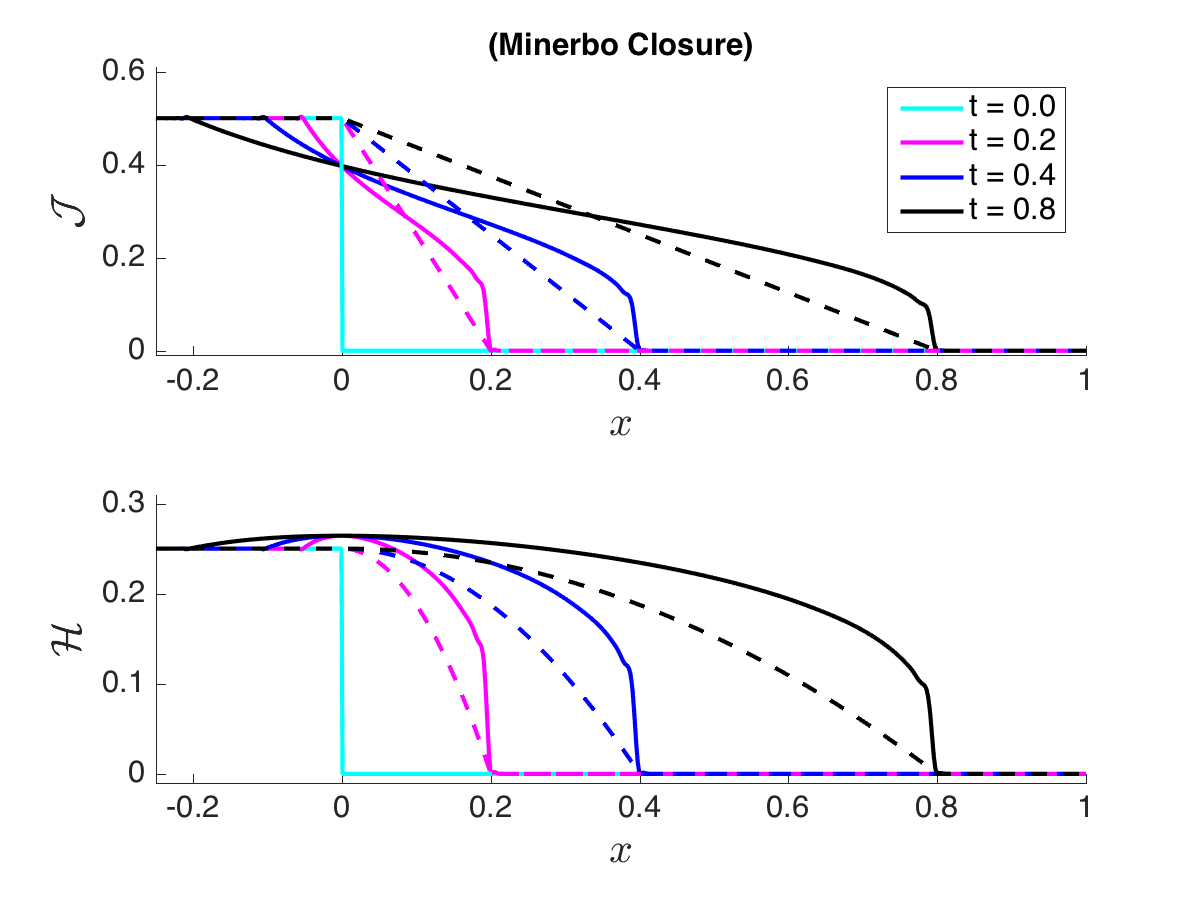
\includegraphics[width=0.5\textwidth]{figures/PackedBeam_ME_MI}
  \end{tabular}
   \caption{Packed Beam}
  \label{fig:PackedBeam}
\end{figure}

\subsection{Line Source}

The line source benchmark (cf. \cite{brunner_2002,garrettHauck_2013}) is a challenging test for approximate transport algorithms.  
In cylindrical coordinates, it consists of an initial delta function particle distribution in radius; i.e., $f_{0}=\delta(R)/4\,\pi$.  
For $t>0$, a cylindrical radiation front propagates radially.  
Apart from capturing details of the exact transport solution, maintaining realizability ($\bcM\in\cR$ cf. Eq.~\eqref{eq:realizableSet}) of the two-moment solution is challenging.  

This test is computed on a two-dimensional domain with $D=\{\vect{x}\in\bbR^{2}:x^{1}\in[0,1.25], x^{2}\in[0,1.25]\}$.  
We follow the initialization procedure in \cite{garrettHauck_2013}, and approximate the initial condition with an isotropic Gaussian distribution function
\begin{equation}
  f_{\mbox{\tiny G},0}
  =\max\Big[\,\f{1}{8\,\pi\,\sigma_{\mbox{\tiny G}}^{2}}\,e^{-R^{2}/(2\,\sigma_{\mbox{\tiny G}}^{2})},10^{-4}\,\Big],
\end{equation}
where $R=|\vect{x}|$, and we use $\sigma_{\mbox{\tiny G}}=0.03$.  
We run this test to a final time $t=1.0$.  

\subsection{Homogeneous Sphere}

The homogeneous sphere test (e.g., \cite{smit_etal_1997}) considers of a sphere with radius $R$.  
Inside the sphere (radius $<R$), the absorption opacity $\sigma_{\Ab}$ and the equilibrium distribution function $f_{0}$ are set to constant values.  
The scattering opacity $\sigma_{\Scatt}$ is set to zero in this test (i.e., $\xi=1$).  
Outside the sphere, the absorption opacity is zero.  
The steady state solution, obtained by solving the transport equation in spherical symmetry, is given by
\begin{equation}
  f_{\mbox{\tiny A}}(r,\mu)=f_{0}\,\big(1-e^{-\chi_{0}\,s(r,\mu)}\big),
  \label{eq:distributionHomogeneousSphere}
\end{equation}
where
\begin{equation}
  s(r,\mu)
  =\left\{
  \begin{array}{lll}
    r\,\mu+R\,g(r,\mu) & \mbox{if}\quad r<R, & \mu\in[-1,+1], \\
    2\,R\,g(r,\mu) & \mbox{if}\quad r \ge R, & \mu\in[(1-(R/r)^{2})^{1/2},+1], \\
    0 & \mbox{otherwise},
  \end{array}
  \right.
\end{equation}
and $g(r,\mu)=[1-(r/R)^{2}(1-\mu^{2})]^{1/2}$.  

\begin{figure}[h]
  \centering
  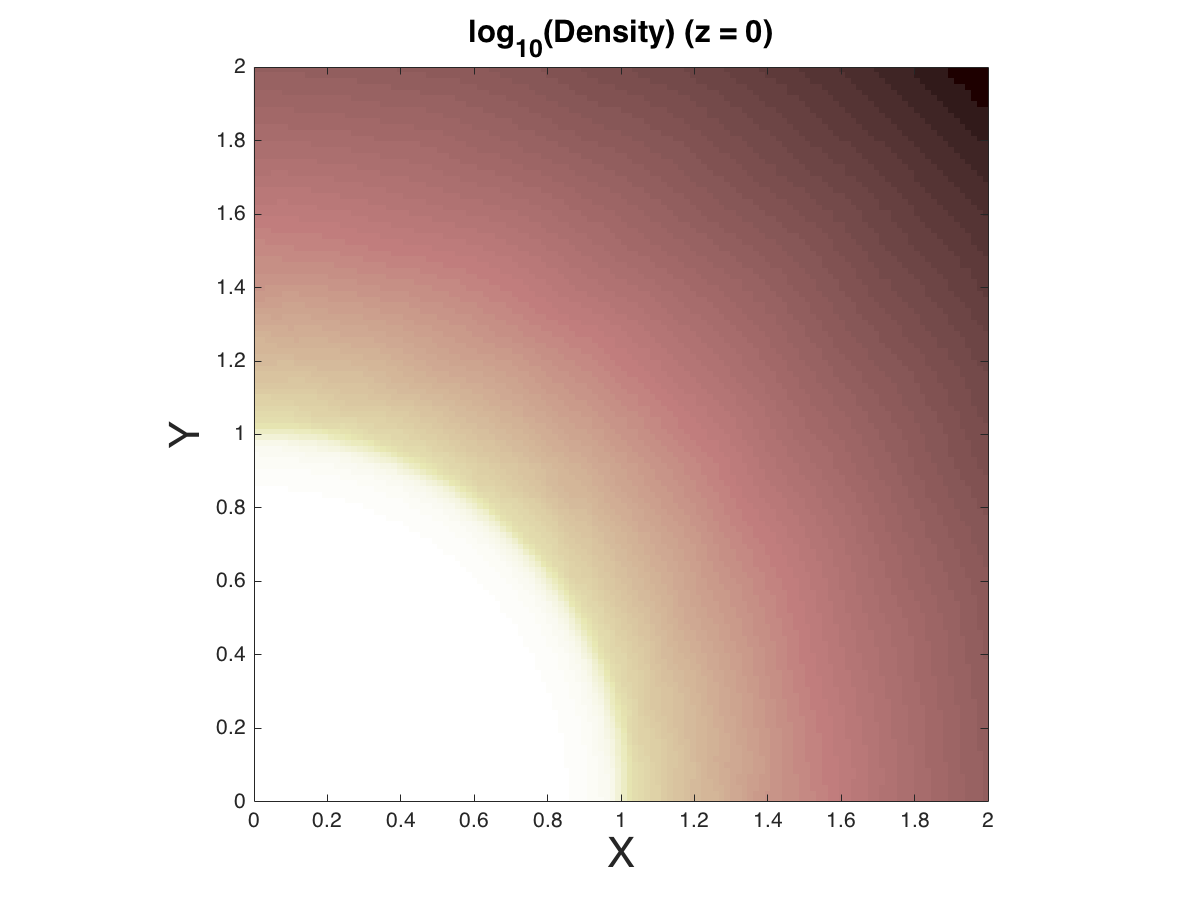
\includegraphics[width=1.0\textwidth]{figures/HomogeneousSphere_Resolution_3}
  \begin{tabular}{cc}
    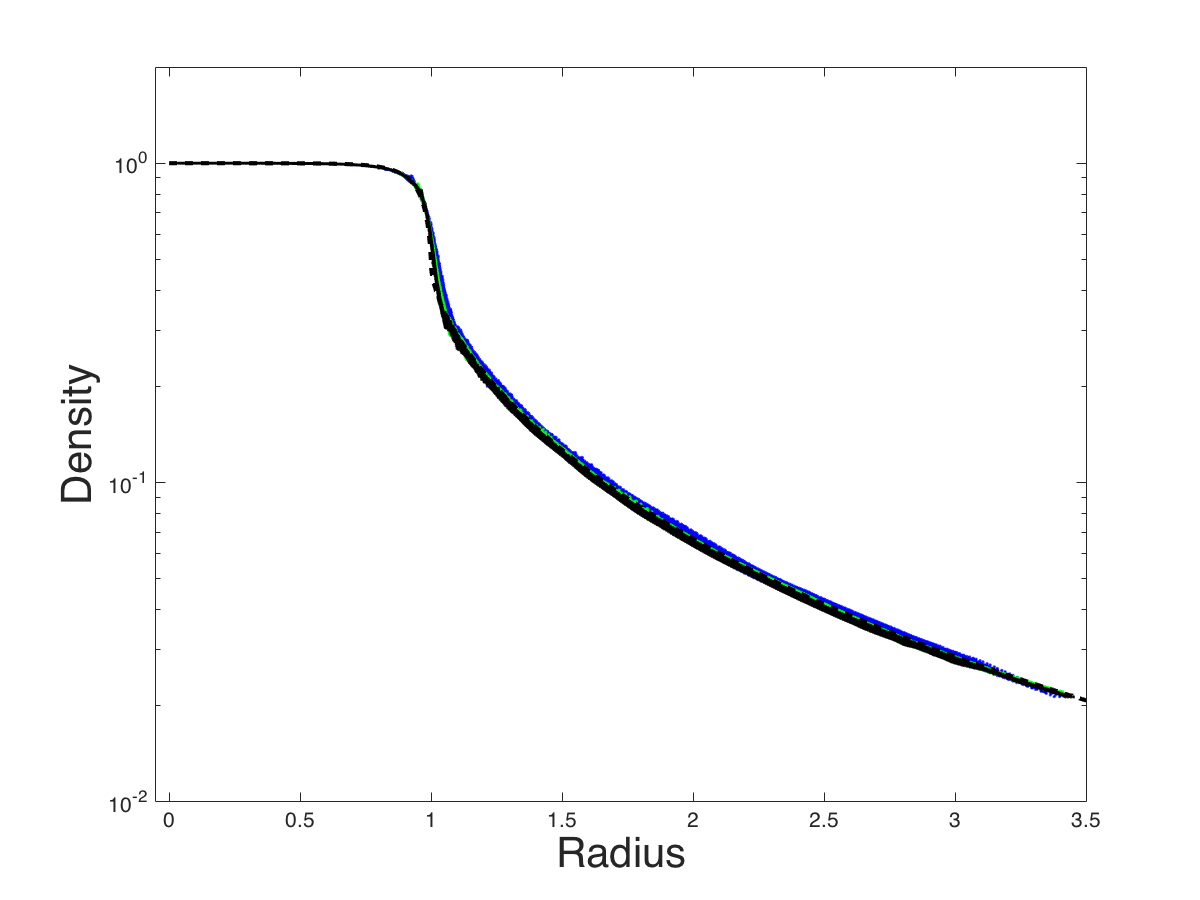
\includegraphics[width=0.5\textwidth]{figures/HomogeneousSphere_Resolution_1}
    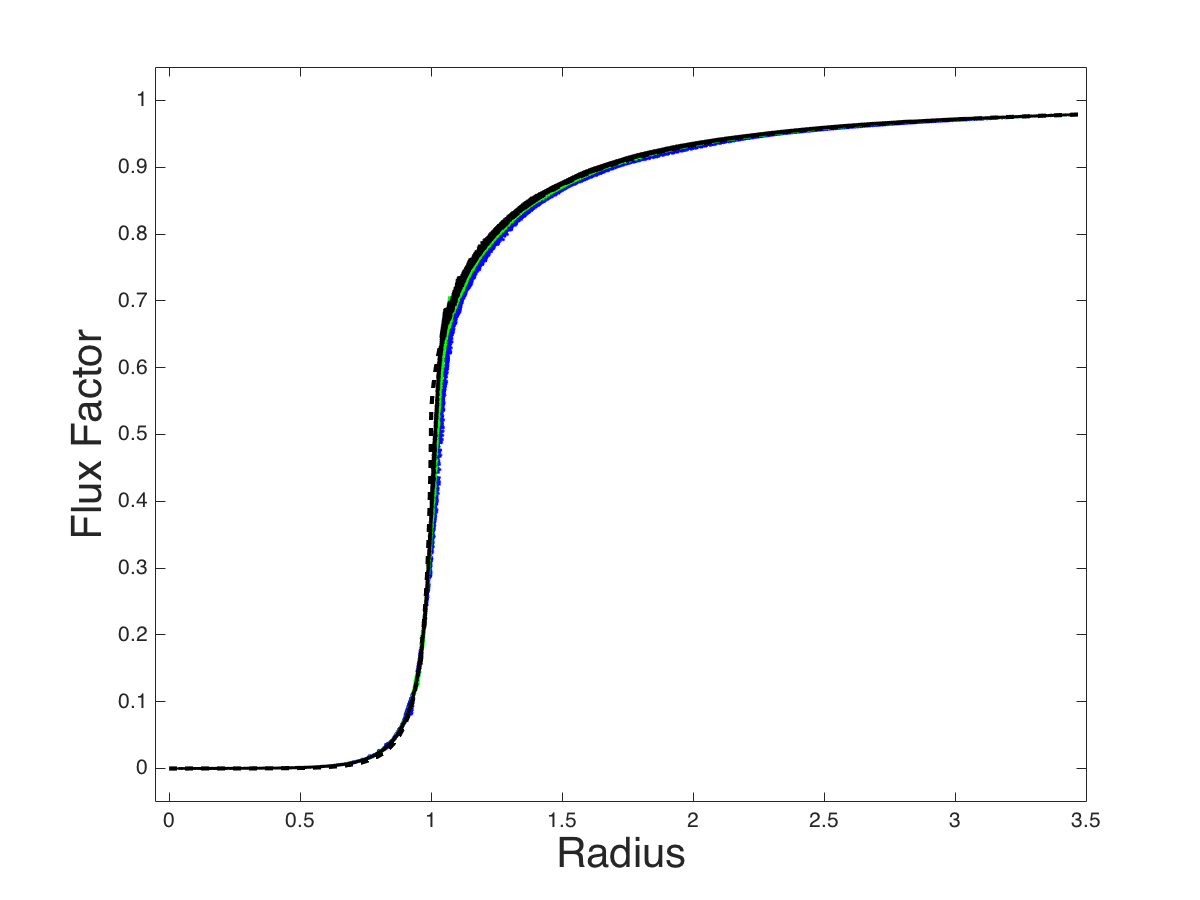
\includegraphics[width=0.5\textwidth]{figures/HomogeneousSphere_Resolution_2}
  \end{tabular}
   \caption{Homogeneous sphere problem: 32$^{3}$, 48$^{3}$, and 64$^{3}$}
  \label{fig:HomogeneousSphere_Resolution}
\end{figure}